% !TeX root = skripta-konstitutivni-vztahy.tex
% !TeX lastmodified = 2018-10-30

\subsection{Víceosé zkoušky elastomerů}
Neplatí princip superpozice a každá složka napětí je funkcí několika složek přetvoření.
Pro obecné vyjádření konstitutivních vlastností materiálu se proto používá měrná energie napjatosti, která je funkcí složek přetvoření.

\begin{figure}[H]
	\centering
	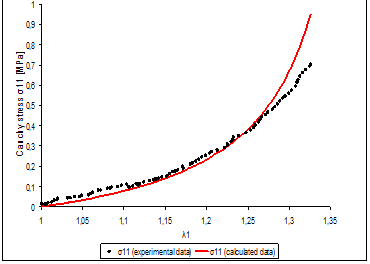
\includegraphics[height=4cm]{jednoosa-tahova-zkouska-tkane}
	\caption{Jednoosá tahová zkouška (měkké biologické tkáně)}
	\label{fig:jednoosa-tahova-zkouska-tkane}
\end{figure}

\begin{figure}[H]
	\centering
	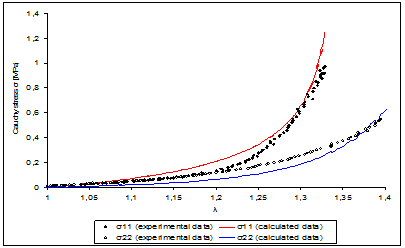
\includegraphics[height=4cm]{dvouosa-tahova-zkouska-tkane}
	\caption{Dvouosá tahová zkouška (měkké biologické tkáně)}
	\label{fig:dvouosa-tahova-zkouska-tkane}
\end{figure}

\subsubsection{Měrná energie napjatosti jako funkce dvou složek přetvoření}
Je tento materiál izotropní?
Jakým typům zkoušek odpovídají experimentální body vyznačené v~obrázku?
\begin{figure}[H]
	\centering
	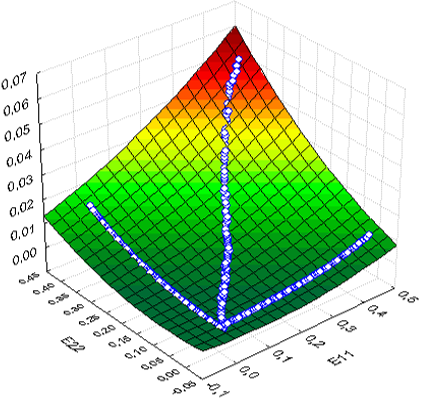
\includegraphics[height=4cm]{merna-energie-napjatosti}
	\caption{Měrná energie napjatosti}
	\label{fig:merna-energie-napjatosti}
\end{figure}

Použitá funkce pro energii napjatosti (Hayashi) má tvar:
\begin{equation}
	W = -C \ln(1-Q),
\end{equation}
kde
\begin{description}
	\item[{$Q = \frac{1}{2} c_1 E_{11}^2 + \frac{1}{2} c_2 E_{22}^2 + c_3 E_{11} E_{22}$}]
	\item[$E_{ii}$] jsou složky Green-Lagrangeova tenzoru přetvoření, 
	\item[{$C [\si{\pascal}]$}] je materiálový parametr definující tuhost materiálu,
	\item[$c_i$] jsou bezrozměrné materiálové parametry.
\end{description}

\subsubsection{Identifikace parametrů měrné energie napjatosti}
Pro identifikaci parametrů je definována funkce ve tvaru
\begin{equation}
	f_w = \sum\limits_{k=1}^n \left(\psi_k - W_k\right)^2,
\end{equation}
kde $\psi_k$ je deformační energie pro $k$-tý bod vypočítaná z~navrženého konstitutivního modelu
\begin{equation}
	\psi_k = \int\limits_0^{E^k_{11}} S_{11} \diff E_{11} + \int\limits_0^{E^k_{22}} S_{22} \diff E_{22}
\end{equation}
a~$W_k$ je deformační energie pro $k$-tý bod vypočítaná z~experimentálních dat pomocí rovnice
\begin{equation}
	W_k = \sum\limits_{j=1}^2 \sum\limits_{i=1}^k \frac{S_{jj}^i + S_{jj}^{i-1}}{2} \left(E_{jj}^i - E_{jj}^{i-1}\right)
\end{equation}

Pro konkrétní tvar konstitutivního modelu (např. logaritmickou funkci uvedenou na předchozí straně) se hledá taková kombinace jejích elastických parametrů, která minimalizuje funkci $f_w$ -- program Hyperfit\footnote{\texttt{http://hyperfit.wz.cz/}}.

\begin{figure}[H]
	\centering
	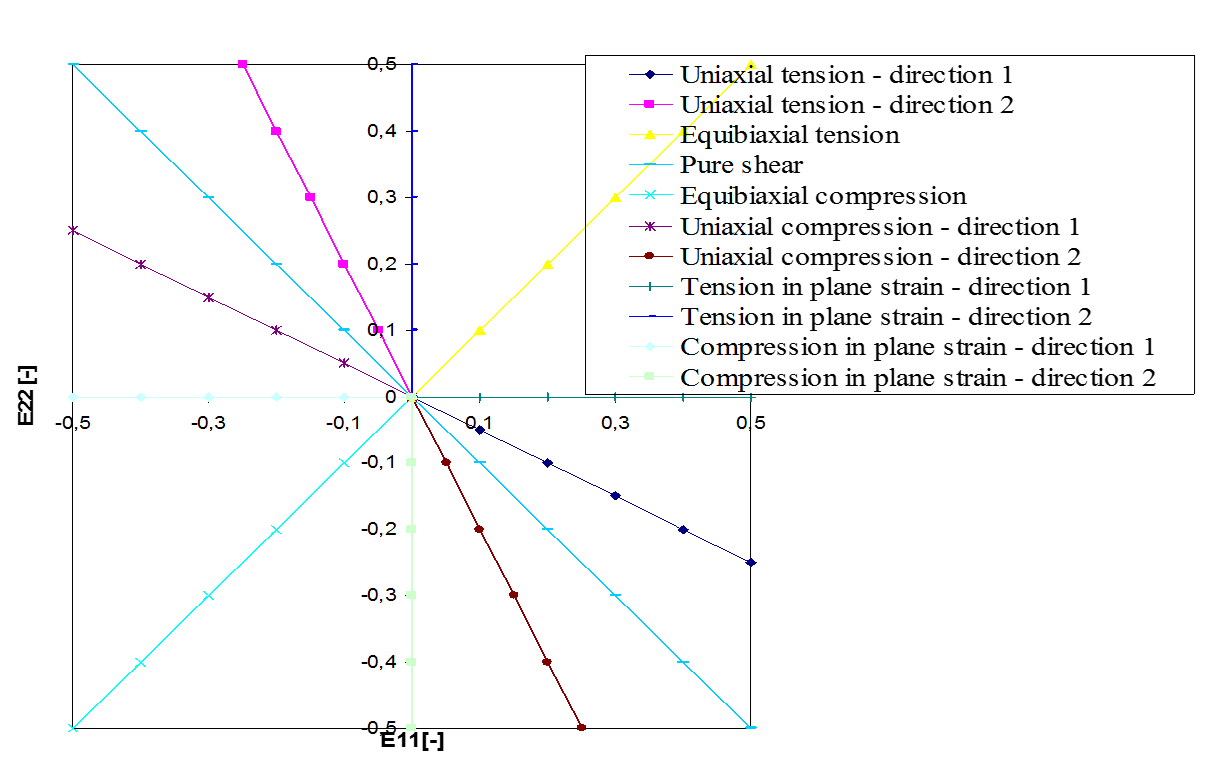
\includegraphics[width=0.6\linewidth]{zkousky-izotropniho-elastomeru}
	\caption[Zkoušky izotropního elastomeru]{Znázornění různých typů zkoušek izotropního elastomeru v~rovině dvou složek přetvoření}
	\label{fig:zkousky-izotropniho-elastomeru}
\end{figure}

\begin{figure}[H]
	\centering
	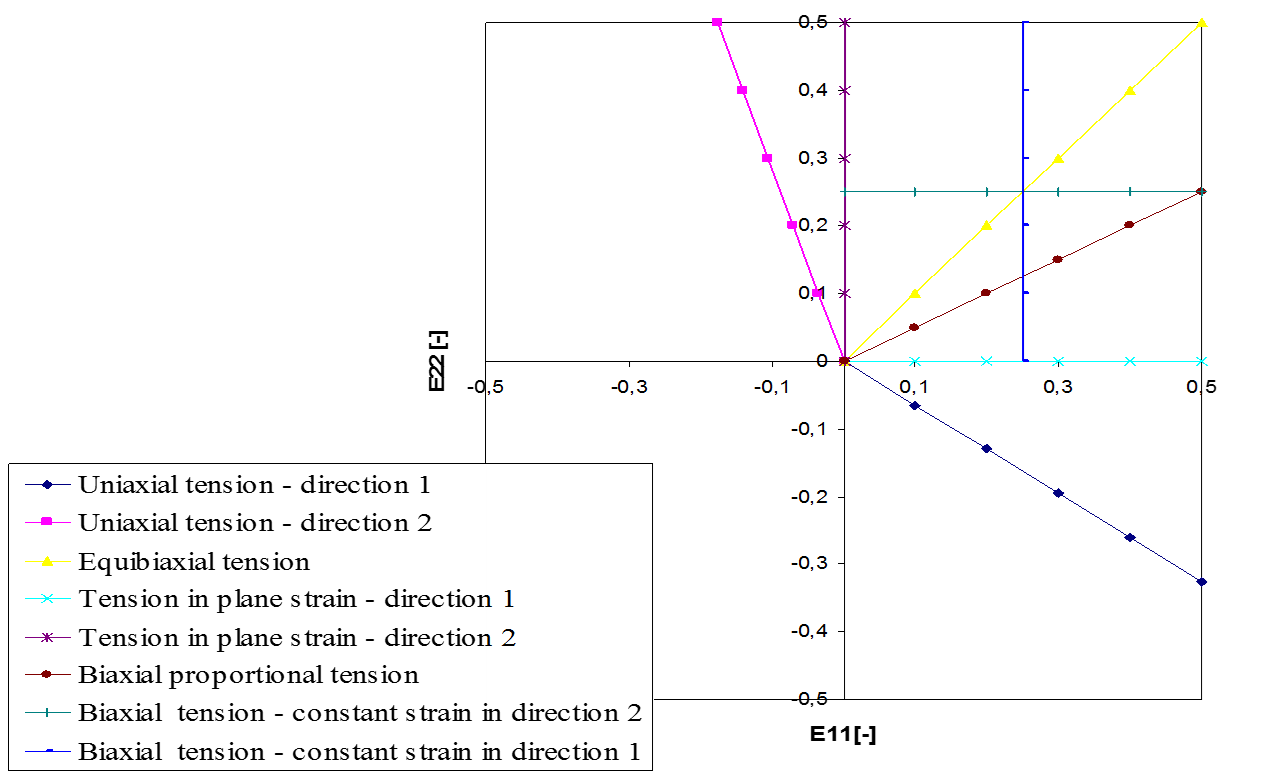
\includegraphics[width=0.6\linewidth]{zkousky-ortotropniho-elastomeru}
	\caption[Zkoušky ortotropního elastomeru]{Znázornění různých typů zkoušek ortotropního elastomeru v~rovině dvou složek přetvoření}
	\label{fig:zkousky-ortotropniho-elastomeru}
\end{figure}

Příklad konstitutivní rovnice ortotropního elastomeru
\begin{equation}
	W = c_1 E_{11}^2 + c_2 E_{11} E_{22} + c_3 E_{22}^2 + c_4 E_{11}^3 + c_5 E_{11}^2 E_{22} + c_6 E_{11} E_{22}^2 + c_7 E_{22}^3
\end{equation}

\begin{figure}[H]
	\centering
	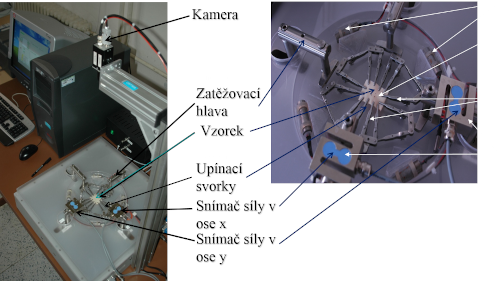
\includegraphics[width=0.7\linewidth]{zkusebni-stroj-elastomeru}
	\caption{Zkušební stroj pro zkoušky elastomerů ve dvouosé napjatosti}
	\label{fig:zkusebni-stroj-elastomeru}
\end{figure}
